\chapter{Índices espectrales}

El objetivo de esta clase es la generación e intepretación de índices espectrales calculados a partir de bandas espectrales de \emph sentinel-2.


\section{Combinación color real}\label{sec:colorreal}

Abra la imagen \begin{center} \directory{S2B\_MSIL2A\_2018-01-31.dim}.
\end{center} seleccione \menu{Open RGB image windows} haciendo click derecho sobre el nombre de la imagen. Se desplegará una nueva ventana (Figura \ref{fig:RGB}) que le permitirá elegir la combinación de bandas. Por defecto aparecerá la combinación color real que utiliza las bandas \emph{rojo (B4)}, \emph{verde(B3)} y \emph{azul(B2)} de \emph{Sentinel-2}. Desplieguela haciendo click en \menu{OK}. 

\section{NDVI}
El NDVI (Normalized Difference Vegetation Index) es uno de los índices más extendidos en teledetección. Utiliza la diferencia entre la absorción de la clorofila en el rojo y la reflectancia del infrarrojo cercano que se relaciona con la biomasa fotosintéticamente activa.

Para calcularlo, seleccione:

\begin{center}
\menu{Optical>Tematic Land Processing > Vegetation Radiometric Indices>NDVI Processor}
  
\end{center}Se desplegará una nueva ventana (Figura \ref{fig:NDVI}). En \menu{Directory} seleccione la carpeta de salida para guardar el archivo en formato BEAM-DIMAP. Seleccione \menu {Run}. El producto ndvi se cargará en \menu{Product Explorer}. Para visualizarlo despliegue con doble click sobre el producto \menu {S2B\_MSIL2A\_2018-01-31>Bands} y seleccione \emph {ndvi}. En el visualizador se desplegará la imagen en escala de grises.

\begin{figure}[h!]
    \centering
    \subfloat[1-I/O Parameters]{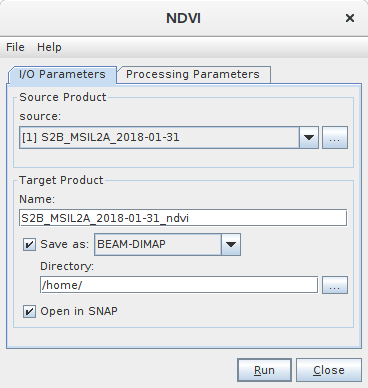
\includegraphics[width=0.4\textwidth]{fig:NDVI.png}\label{fig:NDVI}}
    \hspace{1cm}
    \subfloat[Processing parameters]{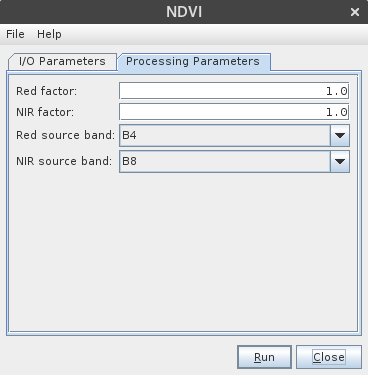
\includegraphics[width=0.4\textwidth]{fig:NDVI-par.png}\label{fig:NDVI-par}}
    \caption{Generacion del \emph{NDVI}.}
    \label{fig:NDVI}
\end{figure}

Identifique los diferentes usos y coberturas (Figura \ref{fig:mapa}) en el producto NDVI. Seleccione alguna cobertura y posicione el cursor en algún pixel de un parche homogéneo. Visualice el valor de \emp {NDVI} para ese parche. Para ello utilice la herramienta  \menu {pixel info}. Desplácece sobre la imagen con el cursor y visualice  los valores que toma el \emph{NDVI} para cada cobertura. Relacione estos valores con la escala de grises de la imagen. 


\section{NDWI}

El NDWI (Normalized Difference Water Index) es un estimador del contenido de agua en el canopeo vegetal que interactua con la radación solar incidente. Es sensible a cambios en el contenido de agua en las hojas. Puede ser utilizado de manera complementaria al NDVI para monitoreo de contenido de agua y estado fisiológico en vegetación. Sin embargo es sensible al ruido del suelo sin cobertura.

Para calcularlo, seleccione \menu{Optical>Tematic Land Processing > Water Radiometric Indices>NDWI Processor}.  Se desplegará una nueva ventana (Figura \ref{fig:NDVI}). En \menu{Directory} seleccione la carpeta de salida para guardar el archivo en formato BEAM-DIMAP. Seleccione \menu {Run}. El producto \emp{NDWI} se cargará en \menu{Product Explorer}. Para visualizarlo despliegue con doble click sobre el producto \menu {S2B\_MSIL2A\_2018-01-31>Bands} y seleccione \emph {ndwi}. En el visualizador se desplegará la imagen en escala de grises. Compare y analice tal como lo hizo con el \emph{NDVI}

\section{SAVI}

El SAVI (Soil Adjusted Vegetation Index)  tal como el NDVI utiliza la diferencia entre la absorción de la clorofila en el rojo y la reflectancia del infrarrojo cercano. Tiene la ventaja de reducir el ruido de la reflectancia del suelo. Además permite ajustar el mismo de acuerdo al tipo de sustrato y porcentaje de cobertura. %re-redactar, está horrible.

Para calcularlo, seleccione \menu{Optical>Tematic Land Processing > Vegetation Radiometric Indices>SAVI Processor}.  Se desplegará una nueva ventana (Figura \ref{fig:NDVI}). En \menu{Directory} seleccione la carpeta de salida para guardar el archivo en formato BEAM-DIMAP. Seleccione \menu {Run}. El producto \emp{SAVI} se cargará en \menu{Product Explorer}. Para visualizarlo despliegue con doble click sobre el producto \menu {S2B\_MSIL2A\_2018-01-31>Bands} y seleccione \emph {savi}. En el visualizador se desplegará la imagen en escala de grises. Compare y analice tal como lo hizo con el \emph{NDVI}.

\section{Visualización con paleta de colores}

Una forma práctica de visualizar productos monobanda como el NDVI o SAVI es utilizando una paleta de colores mediante la cual puede observar los valores bajos con un determinado color, los valores intermedios con otro y así con los valores más altos, permitiendo además un gradiente de colores. %ver redacción

Seleccione en el \menu {Área de visualización} el producto \emph{NDVI}. En \menu {Colour manipulation} podrá ver la distribución estadística de los pixeles del producto (Figura \ref{fig:color-man}). Seleccione la función \menu{import color palette from text file}. En el menú encontrará varias paletas de color, seleccione  \folder{meris\_veg\_index.cpd}. 

\begin{figure}[h!]
    \centering
    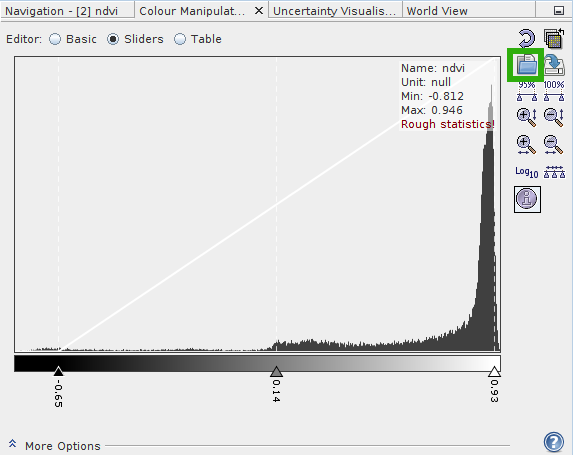
\includegraphics[width=0.6\textwidth]{fig:colour-man.png}
    \caption{Herramienta de Manipulación de Color. En sliders se observa la distribución estadístca de valores de NDVI}
    \label{fig:color-man}
\end{figure}


\section{Actividad práctica II}

%Comparar NDVI entre coberturas
%Comparar NDWI entre coberturas
%Comparar SAVI o GEMI
% Comparar la relacioon GEMI vs NDVI
% Hacer tabla comparativa entre indices

\begin{enumerate}
  \item Identifique parches homogéneos de vegetación, suelo sin cobertura y agua. Compare los valores de \emph{NDVI} utilizando la herramienta \menu{Pixel info}.
  
  
   herramienta \menu{Pin Manager} y grafique con la herramienta \menu{Spectrum View}
\begin{enumerate}
    \item Compare las tres firmas espectrales. Analice el patrón de reflectancia. ¿Presentan todas el mismo patrón?
    \item Identifique picos y valles de reflectancia. ¿Que cuerpo de agua presenta mayor reflectancia en el visible-NIR? ¿Cuál presenta menor? Analice los factores biofísicos que modelan este comportamiento.

  \end{enumerate}

  \item Seleccione entre las pestañas abiertas la que corresponda a la combinación vegetación sana (Sección \ref{sec:vegetacionsana}). Inserte un pin para selva paranaense, bosque implantado, cultivo y suelo sin cobertura vegetal. Modifique el nombre y color de los mismos con la herramienta \menu{Pin Manager} y grafique con la herramienta \menu{Spectrum View}
  \begin{enumerate}
    \item Analice las cuatro firmas espectrales teniendo en cuenta los picos y valles de reflectancia de acuerdo a la longitud de onda correspondiente. ¿En qué longitudes de onda presenta mayor reflectancia la vegetación? ¿En cuáles presenta menor reflectancia? Analice teniendo en cuenta los parámetros fisiológicos que modelan este comportamiento.
    \item Compare una firma de vegetación fotosintéticamente activa (e.g. selva paranaense) con otra de suelo sin cobertura vegetal. ¿Muestra una separación en el visible? ¿Y en el infrarrojo cercano? Analice donde se observan mayores diferencias.
	\item Identifique un área urbana, añada un pin. Modifique nombre y color. Compare con el resto de las firmas espectrales. ¿Que diferencias observa con respecto a suelo sin cobertura vegetal? ¿En qué regiones del espectro las observa? 
  \end{enumerate}
 \end{enumerate}
%Ver cómo manejar el tema de borrar pines en las comparaciones
% Añadir al anexo las longitudes de onda x mision satelital.
 